\documentclass{article}


% Packages
\usepackage{fullpage}
\usepackage{amssymb}
\usepackage{multicol}
\usepackage{amsmath}
\usepackage{amsfonts}
\usepackage{bm}
\usepackage{float}
\usepackage{tikz}
\usepackage{xcolor}
\usetikzlibrary{shapes.geometric, positioning, arrows, intersections}
\tikzset{point/.style={circle,draw=black,inner sep=0pt,minimum size=3pt}}
\usepackage{amsthm}
\usepackage{tcolorbox}
\usepackage{hyperref}
\hypersetup{
    colorlinks=true, %set true if you want colored links
    linktoc=all,     %set to all if you want both sections and subsections linked
    linkcolor=black,  %choose some color if you want links to stand out
}
\usepackage{fancyhdr}


% Macros
\newcommand{\R}{\mathbb{R}}
\newcommand{\N}{\mathbb{N}}
\newcommand{\Q}{\mathbb{Q}}
\newcommand{\sub}{\subset}
\renewcommand{\a}{\alpha}
\renewcommand{\b}{\beta}
\newcommand{\g}{\gamma}
\renewcommand{\d}{\delta}
\newcommand{\e}{\varepsilon}
\newcommand{\ex}{\exists\,}
\newcommand{\overbar}[1]{\mkern 1.5mu\overline{\mkern-1.5mu#1\mkern-1.5mu}\mkern 1.5mu}
\newcommand{\eR}{\overbar{\R}}

%\setlength{\columnsep}{20pt}

%ToC stuff
\newtheorem{example}{Example}
\newtheorem{solution}{Solution}
%\newtheorem{definition}{Definition}[subsection]
\newtheorem{corollary}{Corollary}

\tcbuselibrary{theorems}
\newtcbtheorem[number within=section]{theorem}{Theorem}%
{colback=green!5,colframe=green!35!black,fonttitle=\bfseries}{th}
\newtcbtheorem[number within=section]{definition}{Definition}%
{colback=blue!5,colframe=blue!35!black,fonttitle=\bfseries}{def}

 % Document stuff

\title{Week 3: Differentiation}
\author{James Arthur}

\begin{document}
\maketitle
\tableofcontents
\newpage

\multicols{2}

\section{Definition of a Derivative}
\noindent\begin{definition}{Derivative}{}
   A function $f$, is differentiable at an interior point, $x_0$, of it's domain if the difference qiotient:
   $$ \frac{f(x) - f(x_0)}{x -x_0}, \quad x\neq x_0 $$
   approaches a limit as $x$ approaches $x_0$, in which case the limit is called the {\color{blue} derivative }of $f$ at $x_0$ and is denoted: $f'(x_0)$, thus:
   $$ f'(x_0) = \lim_{x\to x_0}\frac{f(x) - f(x_0)}{x -x_0} $$
\end{definition}\vspace{10pt}

\noindent\begin{definition}{}{}
   We say that $f(x_0)$ is a {\color{blue} local extreme }value of $f$, if there is a $\d > 0$, such that the sign of $f(x) - f(x_0)$ diesnt change:
   $$ (x_0 - \d, \, x_0 + \d) \sub D_f $$
   or a {\color{blue} local minimum } of $f$ if:
   $$ f(x_0) \le f(x) $$
   if for all $x$ in the set, these are true, then we have globals
\end{definition}\vspace{10pt}

\noindent\begin{theorem}{}{}
  If $f$ is differentiable at a local extreme point $x_0 \in D_f^0$, then $f(x_0) = 0$
\end{theorem}\vspace{10pt}
\begin{proof}
  We consider the case where $x_0$ is a local maximum. Then, $\ex \d > 0$, $\displaystyle{(x_0 - \d,\, x_0 + \d) \sub D_f}$ and $f(x) \le f(x_0)$ for all $x\in (x_0-\d,\, x_0+\d)$. We have:
  $$ 0 \le \lim_{x\to x_0-} \frac{f(x) - f(x_0)}{x - x_0} $$
  and
  $$ \lim_{x\to x_0-} \frac{f(x) - f(x_0)}{x - x_0} \le 0$$
  So, as it exists,
  $$ \lim_{x\to x_0-} \frac{f(x) - f(x_0)}{x - x_0} = 0 $$
  The case of a local minimum at $x_0$ is obtained by applying the above to $-f$.
\end{proof}

\section{Rolles Theorem}

\noindent\begin{theorem}{Rolle's Theorem}{}
   Suppose that $f$ is continuous on the closed interval $[a, \, b]$ and differentiable on the open interval $(a, \, b)$ and $f(a) = f(b)$, then $f'(c) = 0$ for some $c\in (a,\,b)$
\end{theorem}\vspace{10pt}

\begin{figure}[H]
  \centering
  \begin{tikzpicture}[scale=1.0]
      \draw[thick, orange] (1,1) node[point,fill=black] (a) {} parabola bend (3,3) (4,2.5) node[point,fill=black] (b) {};
      \draw[white] (1,1+9/8) -- (4,2.5+9/8) coordinate (topright);
      \node[point,fill=black] (x0) at (2.5,2.875) {};

      \coordinate (origin) at (0,0);
      \draw[<->] (topright -| origin) -- (origin) -- (origin -| topright) -- +(1,0);
      \draw[dotted,very thick] (a) -- (a|-origin) node[below,black] {$a$};
      \draw[dotted,very thick] (b) -- (b|-origin) node[below] {$b$};
      \draw[dashed] (x0) -- (x0|-origin) node[below] {$x_0$};
  \end{tikzpicture}
\end{figure}
\begin{proof}
  Since $f$ is continuous on $[a,\, b]$, then, by EVT, $f$ attains both a min and max values.
  $$ \a = \min_{x\in [a,\,b]}{f(x)} \qquad \b = \max_{x\in [a,\,b]}{f(x)} $$
  If $\a = \b$, then $f$ is constant on $(a,\, b)$, clearly $f'(x) = 0 \,\forall x\in [a,\, b]$.\\
  If $\a \neq \b$, then at least one $\a$ or $\b$ is attained at a point $c\in (a,\, b)$ (Since $f(a) = f(b)$), and hence $f'(c) = 0$.
\end{proof}

\section{Darboax's Theorem}


\noindent\begin{theorem}{Darboax's Theorem}{}
  Suppose that $f$ is differentiable on $[a,\, b]$, $f'(a)\neq f'(b)$, and $\mu$ is between $f'(a)$ and $f'(b)$. Then $f'(c) = \mu$ for some $c\in (a,\, b)$.
\end{theorem}\vspace{10pt}
\begin{proof}
  Suppose that $f'(a) < \mu < f'(b)$ aand then define:
  $$ g(x) = f(x) - \mu x $$
  Then
  $$ g'(x) = f'(x) - \mu $$
  and then:
  \begin{equation}
    g'(a) < 0 \qquad 0 < g'(b) \tag{$*$}
  \end{equation}
  Since $g$ is continuous on $[a,\, b]$, $g$ attains a min, by EVT, at some point $c\in [a,\, b]$. Then, ($*$), implies $\ex \d > 0$,
  $$ g(x) < g(a), \quad\forall a < x < a + \d $$
  and
  $$ g(x) < g(b), \quad b - \d < x < b $$
  therefore $c\neq a$ and $c \neq b$. Hence $a < c < b$, and therefore $g'(c) = 0$ since $c$ is a min in $D_g^0$, that is $f'(c)\neq \mu$\\
  The proof when $f'(b)<\mu < f'(a)$ is obtained when you apply the above argument to $-f$.
\end{proof}

\section{Mean Value Theorem}

\noindent\begin{theorem}{Cauchy's Mean Value Theorem}{}
  If $f$ and $g$ are continuous on a closed interval $[a,\, b]$ nd differentiable on the open interval $(a,\, b)$, then:
  $$ [g(b) - g(a)]f'(c) = [f(b) - f(a)]g'(c) $$
  for some $c\in (a,\, b)$
\end{theorem}\vspace{10pt}
\begin{proof}
  Let $h(x) = (g(b) - g(a))f(x)- (f(b) - f(a))g(x)$, then we can say $h$ is continuous on $[a,\, b]$ and differentiable on $(a,\, b)$. Therefore Rolle's Theorem implies that $h'(c) = 0$ for some $c\in (a,\, b)$, that is:
  $$ h'(c) = (g(b) - g(a))f'(c) - (f(b) - f(a))g'(c) = 0 $$
\end{proof}

\noindent\begin{theorem}{Mean Value Theorem}{}
  If $f$ is continuous on the closed interval $[a,\,b]$ and differentiable on $(a,\,b)$, then
  $$ f'(c) = \frac{f(b) - f(a)}{b - a} $$
  for some $c\in (a,\,b)$
\end{theorem}\vspace{10pt}
\begin{figure}[H]
  \centering
  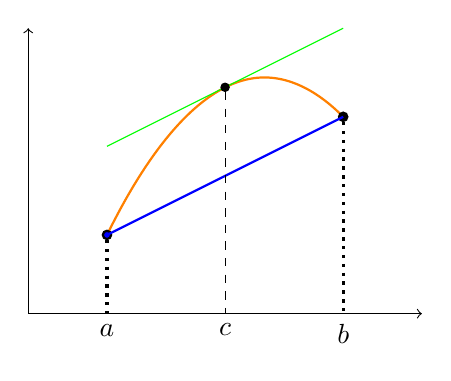
\begin{tikzpicture}[scale=1.0]
      \draw[thick, orange] (1,1) node[point,fill=blue] (a) {} parabola bend (3,3) (4,2.5) node[point,fill=black] (b) {};
      \draw[thick, blue] (1,1) -- (4,2.5);
      \draw[green] (1,1+9/8) -- (4,2.5+9/8) coordinate (topright);
      \node[point,fill=black] (x0) at (2.5,2.875) {};

      \coordinate (origin) at (0,0);
      \draw[<->] (topright -| origin) -- (origin) -- (origin -| topright) -- +(1,0);
      \draw[dotted,very thick] (a) -- (a|-origin) node[below,black] {$a$};
      \draw[dotted,very thick] (b) -- (b|-origin) node[below] {$b$};
      \draw[dashed] (x0) -- (x0|-origin) node[below] {$c$};
  \end{tikzpicture}
\end{figure}
\begin{proof}
  Apply Cauchy MVT and let $g(x) = x$
\end{proof}
\subsection{Consequences}
\noindent\begin{theorem}{}{}
 If $f'(x) = 0$ for all $x\in (a,\,b)$ then $f$ is constant on $(a\,b)$.
\end{theorem}\vspace{10pt}
\noindent\begin{theorem}{}{}
 If $f'$ exists and does not change sign on $(a,\,b)$, then $f$ is monotonic on $(a,\,b)$
\end{theorem}\vspace{10pt}
\noindent\begin{theorem}{Lipschitz Continuity}{}
 If $|f'(x)|\le M \quad\forall x\in(a,\,b)$, then $|f(x) - f(x')| < M|x - x'|$ for all $x, x' \in (a,\,b)$.
\end{theorem}\vspace{10pt}
















\end{document}
